%----------------------------------------------------------------------------------------
%	PACKAGES AND OTHER DOCUMENT CONFIGURATIONS
%----------------------------------------------------------------------------------------

\documentclass{article}

\usepackage{fancyhdr} % Required for custom headers
\usepackage{lastpage} % Required to determine the last page for the footer
\usepackage{extramarks} % Required for headers and footers
\usepackage[usenames,dvipsnames]{color} % Required for custom colors
\usepackage{graphicx} % Required to insert images
\usepackage{listings} % Required for insertion of code
\usepackage{courier} % Required for the courier font
\usepackage{lipsum} % Used for inserting dummy 'Lorem ipsum' text into the template
\usepackage{amsmath} % Required for align
\usepackage{enumerate} % Enumerate
\usepackage{amsfonts}
\DeclareMathOperator{\Ima}{im}

% Margins
\topmargin=-0.45in
\evensidemargin=0in
\oddsidemargin=0in
\textwidth=6.5in
\textheight=9.0in
\headsep=0.25in

\linespread{1.1} % Line spacing

% Set up the header and footer
\pagestyle{fancy}
\lhead{\hmwkAuthorName} % Top left header
\chead{\hmwkClass\ (\hmwkClassInstructor): \hmwkTitle} % Top center head
\rhead{\firstxmark} % Top right header
\lfoot{\lastxmark} % Bottom left footer
\cfoot{} % Bottom center footer
\rfoot{Page\ \thepage\ of\ \protect\pageref{LastPage}} % Bottom right footer
\renewcommand\headrulewidth{0.4pt} % Size of the header rule
\renewcommand\footrulewidth{0.4pt} % Size of the footer rule

\setlength\parindent{0pt} % Removes all indentation from paragraphs

%----------------------------------------------------------------------------------------
%	CODE INCLUSION CONFIGURATION
%----------------------------------------------------------------------------------------

\definecolor{MyDarkGreen}{rgb}{0.0,0.4,0.0} % This is the color used for comments
\lstloadlanguages{Perl} % Load Perl syntax for listings, for a list of other languages supported see: ftp://ftp.tex.ac.uk/tex-archive/macros/latex/contrib/listings/listings.pdf
\lstset{language=Perl, % Use Perl in this example
  frame=single, % Single frame around code
  basicstyle=\small\ttfamily, % Use small true type font
  keywordstyle=[1]\color{Blue}\bf, % Perl functions bold and blue
  keywordstyle=[2]\color{Purple}, % Perl function arguments purple
  keywordstyle=[3]\color{Blue}\underbar, % Custom functions underlined and blue
  identifierstyle=, % Nothing special about identifiers                                         
  commentstyle=\usefont{T1}{pcr}{m}{sl}\color{MyDarkGreen}\small, % Comments small dark green courier font
  stringstyle=\color{Purple}, % Strings are purple
  showstringspaces=false, % Don't put marks in string spaces
  tabsize=5, % 5 spaces per tab
        %
        % Put standard Perl functions not included in the default language here
  morekeywords={rand},
        %
        % Put Perl function parameters here
  morekeywords=[2]{on, off, interp},
        %
        % Put user defined functions here
  morekeywords=[3]{test},
        %
  morecomment=[l][\color{Blue}]{...}, % Line continuation (...) like blue comment
  numbers=left, % Line numbers on left
  firstnumber=1, % Line numbers start with line 1
  numberstyle=\tiny\color{Blue}, % Line numbers are blue and small
  stepnumber=5 % Line numbers go in steps of 5
}


%----------------------------------------------------------------------------------------
%	DOCUMENT STRUCTURE COMMANDS
%	Skip this unless you know what you're doing
%----------------------------------------------------------------------------------------

% Header and footer for when a page split occurs within a problem environment
\newcommand{\enterProblemHeader}[1]{
  \nobreak\extramarks{#1}{#1 continued on next page\ldots}\nobreak
  \nobreak\extramarks{#1 (continued)}{#1 continued on next page\ldots}\nobreak
}

% Header and footer for when a page split occurs between problem environments
\newcommand{\exitProblemHeader}[1]{
  \nobreak\extramarks{#1 (continued)}{#1 continued on next page\ldots}\nobreak
  \nobreak\extramarks{#1}{}\nobreak
}

\setcounter{secnumdepth}{0} % Removes default section numbers
\newcounter{homeworkProblemCounter} % Creates a counter to keep track of the number of problems

\newcommand{\homeworkProblemName}{}
\newenvironment{homeworkProblem}[1][Problem \arabic{homeworkProblemCounter}]{ % Makes a new environment called homeworkProblem which takes 1 argument (custom name) but the default is "Problem #"
  \stepcounter{homeworkProblemCounter} % Increase counter for number of problems
  \renewcommand{\homeworkProblemName}{#1} % Assign \homeworkProblemName the name of the problem
  \section{\homeworkProblemName} % Make a section in the document with the custom problem count
  \enterProblemHeader{\homeworkProblemName} % Header and footer within the environment
}{
  \exitProblemHeader{\homeworkProblemName} % Header and footer after the environment
}

\newcommand{\problemAnswer}[1]{ % Defines the problem answer command with the content as the only argument
  \noindent\framebox[\columnwidth][c]{\begin{minipage}{0.98\columnwidth}#1\end{minipage}} % Makes the box around the problem answer and puts the content inside
}

\newcommand{\homeworkSectionName}{}
\newenvironment{homeworkSection}[1]{ % New environment for sections within homework problems, takes 1 argument - the name of the section
  \renewcommand{\homeworkSectionName}{#1} % Assign \homeworkSectionName to the name of the section from the environment argument
  \subsection{\homeworkSectionName} % Make a subsection with the custom name of the subsection
  \enterProblemHeader{\homeworkProblemName\ [\homeworkSectionName]} % Header and footer within the environment
}{
  \enterProblemHeader{\homeworkProblemName} % Header and footer after the environment
}

%----------------------------------------------------------------------------------------
%	NAME AND CLASS SECTION
%----------------------------------------------------------------------------------------

\newcommand{\hmwkTitle}{HW 1} % Assignment title
\newcommand{\hmwkDueDate}{Monday,\ January\ 1,\ 2012} % Due date
\newcommand{\hmwkClass}{CS 5220} % Course/class
\newcommand{\hmwkClassTime}{} % Class/lecture time
\newcommand{\hmwkClassInstructor}{Bindel} % Teacher/lecturer
\newcommand{\hmwkAuthorName}{Nicholas Booher, Shuai \\Jiang, Sepehr Saroukhani} % Your name

% Listings 
\usepackage{listings}
\usepackage{color}

\definecolor{dkgreen}{rgb}{0,0.6,0}
\definecolor{gray}{rgb}{0.5,0.5,0.5}
\definecolor{mauve}{rgb}{0.58,0,0.82}

\lstset{frame=tb,
  language=C,
  aboveskip=3mm,
  belowskip=3mm,
  showstringspaces=false,
  columns=flexible,
  basicstyle={\small\ttfamily},
  numbers=none,
  numberstyle=\tiny\color{gray},
  keywordstyle=\color{blue},
  commentstyle=\color{dkgreen},
  stringstyle=\color{mauve},
  breaklines=true,
  breakatwhitespace=true
  tabsize=3
}



%----------------------------------------------------------------------------------------

\begin{document}
  Our first step to optimizing the program was to jump directly into SSE by using the example script already written in Bitbucket.
  The hope was that the SSE code was a fast enough kernel that we can build a good multiplier around it; indeed, it an immediate
  speed-up was noticed! It approximately doubled our naive multiplication. See figure~\ref{fig:initial}.

  \begin{figure}[h]
    \centering
    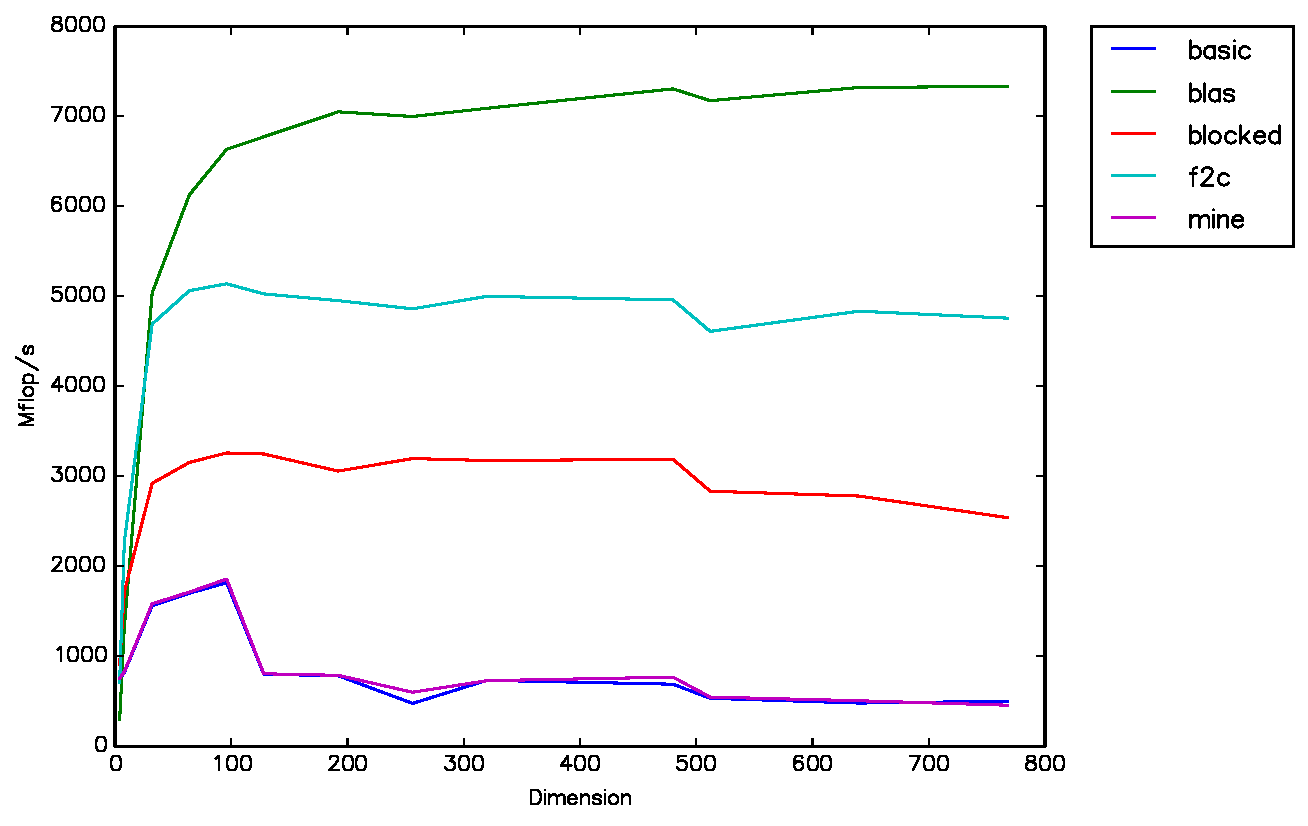
\includegraphics[width=.7\textwidth]{initial.pdf}
    \caption{Our initial set-up using the SSE code provided. Note that due to laziness, the ``blocked'' line is actually our matrix multiply.}
    \label{fig:initial}
  \end{figure}

  What the code does is fairly basic:
  \begin{enumerate}
    \item Intialize arrays At, Bt.
    \item Takes in matrix A, B and copies them into At, Bt such that we have memory layout of 2 by P blocks in A and P by 2 blocks in B.
    \item Loop over the blocks in A and B and multiply, adding the 2 by 2 matrix from the output into the C matrix.
  \end{enumerate}

  We originally compiled this SSE code via the Intel compiler, but weirdly we found that compiling it with the GCC compiler results in a roughly
  33\% speedup over the Intel compiler! We're actually not sure why, but various flags of the ICC doesn't seem to coax the same performance
  out of the code.

  This was all tested on even sizes intially, as there was no need to pad the matrices with anything. The odd cases
  are handled in the natural way, which was to pad a row and column and take the slight hit to the performance.
  When implemented, our performance was still pretty decent. See figure~\ref{fig:odd}.

  \begin{figure}[h]
    \centering
    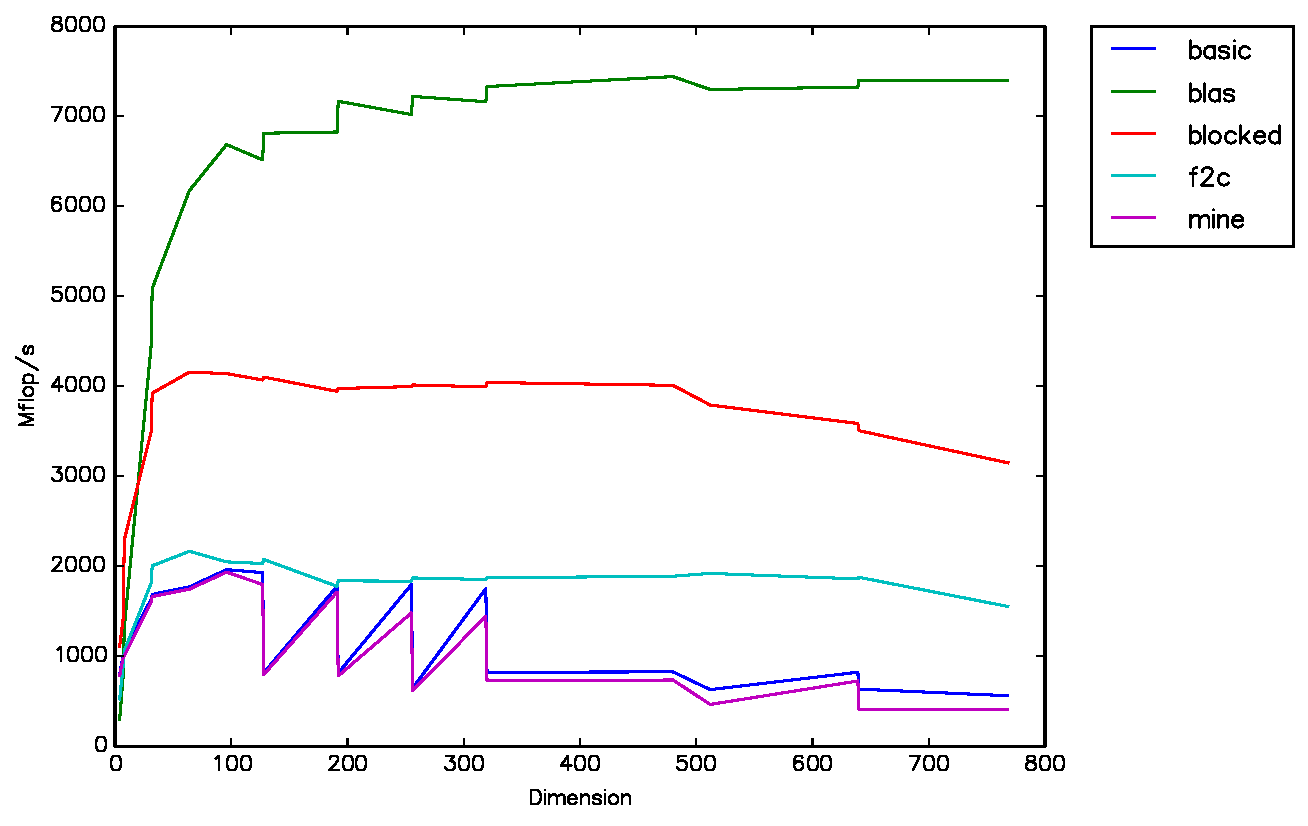
\includegraphics[width=.7\textwidth]{odd.pdf}
    \caption{After adding the odd cases in (note the ``blocked'' line is ours).}
    \label{fig:odd}
  \end{figure}

  The next step to optimizing this was to play with the flags and use tiny code tricks.

  \subsection{Tricks}
    One trick that we played with was to do some loop reordering. In our main block, we have the following

    \begin{lstlisting}
    for (bi = 0; bi < n_blocks; ++bi) {
      const int i = bi * BLOCK_SIZE;
      for (bj = 0; bj < n_blocks; ++bj) {
        const int j = bj * BLOCK_SIZE;
        // trans is our ``transitional'' matrix which contains both At and Bt
        kdgemm2P2(n, tempC, &trans[bi*n*2], &trans[temp + bj*n*2]);
      }
    }
    \end{lstlisting}

    We noted that flipping bi and bj's loop order hurts the performance a lot. For example, at the far end of the spectrum of the sizes
    the different is quite noticable. See table~\ref{tab:looporder}, so we determined that 

    \begin{table}
      \centering
      \begin{tabular}{r c c}
        Size & MFlops (flipped) & MFlops (as shown) \\
        767  & 2660.82 & 3516.27\\
        768  & 2348.95 & 3586.11\\
        769  & 2229.79 & 3503.37
      \end{tabular}
      \caption{Table of loop ordering}
      \label{tab:looporder}
    \end{table}

    Loop reordering was also applied to the copy commands:
    \begin{lstlisting}
    if (odd == 0) {
      for (int j = 0; j<n; j++) {
        for (int i = 0; i < m; i++) {
          At[i*n*2 + 2*j]     = A[j*n + i*2];
          At[i*n*2 + 2*j + 1] = A[j*n + i*2 + 1];
        }
      }
    }
    \end{lstlisting}

    while it wasn't obvious which order should be better as At increments via j via A increments via i, it turns out j, i ordering is \emph{slightly} faster.

    Another small speed increase laid with the serial performance of the copying. Initially, we actually declared to different arrays, one for A and one for B.
    We find that if we just create one giant array of size $2n^2$, and copy A, B into that giant array, performance increase slightly.

    \subsection{Compiler Flags (Sep)}

    \subsection{Memory Usage}

    One thing we tried was to break up the P by 2 and 2 by P matrices into smaller block. Theoretically, since the size of a double is 8 bytes, we need to fit
    $2(2P)*8 + 4 = 32P + 4$ bytes into the cache. While the level 1 cache of the educational nodes are quite low, it seems to not matter from the plots (our maximum
    size that we can fit in the L1 cache is $P=128$). If we look at the level 2 cache, our array size can go up to 1024 theoretically, which (theoretically) shouldn't
    impede us.

    If we look at the cachegrind output for our program, we see the following:
    \begin{lstlisting}
[sj423@en-cluster02 matmul]$ valgrind --tool=cachegrind ./matmul-blocked
==18730== Cachegrind, a cache and branch-prediction profiler
==18730== Copyright (C) 2002-2013, and GNU GPL'd, by Nicholas Nethercote et al.
==18730== Using Valgrind-3.9.0 and LibVEX; rerun with -h for copyright info
==18730== Command: ./matmul-blocked
==18730== 
--18730-- warning: L3 cache found, using its data for the LL simulation.
--18730-- warning: pretending that LL cache has associativity 24 instead of actual 16
Compiler:	gcc
Options:	-O3 -funroll-loops -msse4.2 -ffast-math -mtune=generic -march=corei7
Description:	Simple blocked dgemm.

==18730== 
==18730== I   refs:      62,147,347,847
==18730== I1  misses:             1,539
==18730== LLi misses:             1,518
==18730== I1  miss rate:           0.00%
==18730== LLi miss rate:           0.00%
==18730== 
==18730== D   refs:      32,109,636,396  (27,962,135,435 rd   + 4,147,500,961 wr)
==18730== D1  misses:     1,976,702,658  ( 1,966,158,637 rd   +    10,544,021 wr)
==18730== LLd misses:         7,256,578  (     5,016,816 rd   +     2,239,762 wr)
==18730== D1  miss rate:            6.1% (           7.0%     +           0.2%  )
==18730== LLd miss rate:            0.0% (           0.0%     +           0.0%  )
==18730== 
==18730== LL refs:        1,976,704,197  ( 1,966,160,176 rd   +    10,544,021 wr)
==18730== LL misses:          7,258,096  (     5,018,334 rd   +     2,239,762 wr)
==18730== LL miss rate:             0.0% (           0.0%     +           0.0%  )
    \end{lstlisting}

    which actually mimics the performance of the BLAS cache stats:

    \begin{lstlisting}
[sj423@en-cluster02 matmul]$ valgrind --tool=cachegrind ./matmul-blas 
==1449== Cachegrind, a cache and branch-prediction profiler
==1449== Copyright (C) 2002-2013, and GNU GPL'd, by Nicholas Nethercote et al.
==1449== Using Valgrind-3.9.0 and LibVEX; rerun with -h for copyright info
==1449== Command: ./matmul-blas
==1449== 
--1449-- warning: L3 cache found, using its data for the LL simulation.
--1449-- warning: pretending that LL cache has associativity 24 instead of actual 16
Compiler:	gcc
Options:	-O3 -funroll-loops -msse4.2 -ffast-math -mtune=generic -march=corei7
Description:	System CBLAS dgemm.

==1449== 
==1449== I   refs:      59,157,389,231
==1449== I1  misses:             2,399
==1449== LLi misses:             2,297
==1449== I1  miss rate:           0.00%
==1449== LLi miss rate:           0.00%
==1449== 
==1449== D   refs:      30,847,547,276  (26,700,497,225 rd   + 4,147,050,051 wr)
==1449== D1  misses:     1,670,642,244  ( 1,665,753,557 rd   +     4,888,687 wr)
==1449== LLd misses:         3,023,479  (     2,584,556 rd   +       438,923 wr)
==1449== D1  miss rate:            5.4% (           6.2%     +           0.1%  )
==1449== LLd miss rate:            0.0% (           0.0%     +           0.0%  )
==1449== 
==1449== LL refs:        1,670,644,643  ( 1,665,755,956 rd   +     4,888,687 wr)
==1449== LL misses:          3,025,776  (     2,586,853 rd   +       438,923 wr)
==1449== LL miss rate:             0.0% (           0.0%     +           0.0%  )
    \end{lstlisting}

    Note that it's a similar miss rate in terms of percentages, but our algorithm had to
    use much more read/writes than the BLAS algorithm, which contributes to inefficiencies.

    \subsection{SSE (Nick)}

\end{document}
